\chapter{Implémentation des algorithmes AS/ACS pour le problème SAT}
	\section{Structures de données:}
	\paragraph{}
	Vu les très bonnes performance réalisée par les structures de donnée vues dans \ref{part1}, nous avons logiquement opté pour les même représentations pour l'implémentation d'AS/ACS, à savoir : 
	\subsection{Représentation d’instance et de solutions SAT:}
	\paragraph{}
	\begin{flalign*}
	x_{1} \lor \neg x_{2} \lor x_{4} \\
	\neg x_{2} \lor x_{3} \lor x_{4} \\
	\neg x_{1} \lor x_{2} \lor \neg x_{3}
	\end{flalign*}
	Et la solution suivante:\\
	\begin{center}
		$x_{1} \leftarrow true$, $x_{2} \leftarrow false$, $x_{3} \leftarrow true$, $x_{4} \leftarrow false $
	\end{center}
	
	La représentation:\\
	
	\definecolor{green}{rgb}{0.5,1,0.5}
	\begin{center}
		\begin{tabular}{|c | c| c| c| c|}
			\hline
			$x_{1}$& $x_{2}$ &$x_{3}$ &$x_{4}$ \\\hline
			1 & 0 & 1 & 0 \\\hline
		\end{tabular}\\
		Solution
	\end{center}
	\begin{minipage}{0.5\textwidth}
		\centering
		\begin{tabular}{|c | c| c| c|}
			\hline
			\rowcolor{green}
			$x_{1}$& 1 & 0 & 0 \\\hline
			$x_{2}$& 0 & 0 & 1 \\\hline
			\rowcolor{green}
			$x_{3}$& 0 & 1 & 0 \\\hline
			$x_{4}$& 1 & 1 & 0 \\\hline
		\end{tabular}
	\end{minipage}
	\hfillx
	\begin{minipage}{0.5\textwidth}
		\centering
		\begin{tabular}{|c | c| c| c|}
			\hline
			$\neg x_{1}$& 0 & 0 & 1 \\\hline
			\rowcolor{green}
			$\neg x_{2}$& 1 & 1 & 0 \\\hline
			$\neg x_{3}$& 0 & 0 & 1 \\\hline
			\rowcolor{green}
			$\neg x_{4}$& 0 & 0 & 0 \\\hline
		\end{tabular}
	\end{minipage}\\
	\begin{center}
		Instance
	\end{center}
	On peut calculer les clauses satisfaites par la solution en utilisant le or logique entre les Bitset de ses littéraux:
	\begin{center}
		\begin{minipage}{0.5\textwidth}
			\centering
			\begin{tabular}{| c| c| c|c|}
				\hline
				$x_{1}$& 1 & 0 & 0 \\\hline
			\end{tabular}
		\end{minipage}
		\\~\\
		OR
		\\~\\
		\begin{minipage}{0.5\textwidth}
			\centering
			\begin{tabular}{|c | c| c| c|}
				\hline
				$x_{3}$& 0 & 1 & 0 \\\hline
			\end{tabular}
		\end{minipage}
		\\~\\
		OR
		\\~\\
		\begin{minipage}{0.5\textwidth}
			\centering
			\begin{tabular}{| c| c| c|c|}
				\hline
				$\neg x_{2}$& 1 & 1 & 0 \\\hline
			\end{tabular}
		\end{minipage}
		\\~\\
		OR
		\\~\\
		\begin{minipage}{0.5\textwidth}
			\centering
			\begin{tabular}{|c | c| c| c|}
				\hline
				$\neg x_{4}$& 0 & 0 & 0 \\\hline
			\end{tabular}
		\end{minipage}
		\begin{center}
			
			$\downarrow$
			\\~\\
			\begin{tabular}{|c | c| c| c|}
				\hline
				$Bitset$ résultat& 1 & 1 & 0 \\\hline
			\end{tabular}
		\end{center}
	\end{center}
	
	
	\subsection{La table des Phéromones}
	\paragraph{}
	La différence entre BSO et ACO réside dans le fait qu'une solution n'est pas obtenue selon le voisinage d'une autre solution, mais est construite pas à pas selon une règle de transition d'un état à un autre. Pour garder trace des phéromones déposées par les fourmis lors de la construction de leur solutions respectives, nous pouvons utilisée un tableau a deux dimensions(Matrice) dont les lignes sont les variables de la solution, et les colonnes les deux litéraux de la variable associée. le schéma suivant traduit cela : 
	
	\begin{minipage}{\textwidth}
		\centering
		\begin{table}[H]
			\centering
			\begin{tabular}{|c|c|c|}
				\hline
				$i$ & $x_{i}$ & $\lnot x_{i}$ \\ \hline
				1   & 0.1     & 0.1           \\ \hline
				2   & 0.1     & 0.1           \\ \hline
				3   & 0.1     & 0.1           \\ \hline
				4   & 0.1     & 0.1           \\ \hline
			\end{tabular}
			\caption{Table des phéromones initiale}
		\end{table}
		$\Downarrow$
		\begin{table}[H]
			\centering
			\begin{tabular}{|c|c|c|}
				\hline
				$i$ & $x_{i}$ & $\lnot x_{i}$ \\ \hline
				1   & 0.1     & 0.1           \\ \hline
				2   & 0.1     & 0.1           \\ \hline
				3   & 0.1     & 0.1           \\ \hline
				4   & \cellcolor{green}0.325     & \cellcolor{red!60}0.102           \\ \hline
			\end{tabular}
			\caption{Table des phéromones après le passage d'une fourmi}
		\end{table}
	\end{minipage}
	\\~\\
	La figure illustre le processus de dépôt de phéromones, celui de l'évaporation sera vu plus tard car il dépend du choix de l'algorithme dérivant d'ACO(i.e soi AS ou bien ACS).
	\section{Conception et pseudo-code:}
	\paragraph{}
	L'algorithme ACO a une structure de base très simple, elle se résume à l'algorithme suivant : 
	\begin{algorithm}
		\SetAlgoLined
		\KwResult{retourne la meilleure solution trouvée}
		\textbf{init}($pheromons$)\;
		\textbf{init}($allParameters$)\;
		$meilleureSolution \gets randomSolution$\;
		\While{$\neg$\textbf{fin()}}{
			\ForEach{$fourmi \in fourmis$}
			{
				\textbf{contruireSolution($fourmi$)}\;
				\If{$isValide(fourmi.solution)$ }{
					\Return $fourmi.solution$\;
				}
			}
			\textbf{postConstructionActions($fourmis$)}\;
			\tcp{sera vu plus en détails dans AS/ACS}\;
			\If{\textbf{bestSolution}($fourmis$)>$meilleureSolution$}{
					$meilleureSolution \gets$ \textbf{bestSolution($fourmis$)}\;		
				}
				\textbf{miseAjourt}($pheromons$)\;
			}
		\Return $meilleureSolution$\;
		\caption{Algorithme de recherche ACO}
	\end{algorithm}\\
	\newpage
	\paragraph{}
	Maintenant que nous avons vu le principale fonctionnement d'ACO, il est temps de spécifier le comportement d'AS et ACS:
	\subsection{AS(Ant System)}
	Il repose comme cité dans \ref{AS} sur une règle de transition probabiliste que l'on va détailler après avoir montré le pseudo code suivant : 
	
	\begin{algorithm}[H]
		\SetAlgoLined
		\KwResult{retourne la meilleure solution trouvée}
		\textbf{init}($pheromons$)\;
		\textbf{init}($allParameters$)
		$meilleureSolution \gets randomSolution$\;
		\lFor{$t=1$ \KwTo maxItter}{
			\ForEach{$fourmi\in fourmis$}
			{
				\Repeat{$fourmil$ construit sa solution}
				{
					$P_{i,j} \gets$ \textbf{calculerProba()}\;
					$nextState \gets $ \textbf{selectNextBy($P_{i,j}$)}\; 
				}
				$evaluation$ = \textbf{evaluer($fourmlle.solution$)}\;
				\If{$evaluation$ = $bestScore$}{
					\Return $fourmi.solution$\;
				}
				\textbf{onlinePheromonsUpdate($pheromons$)}\;
			}
			\If{\textbf{bestSolution}($fourmis$)>$meilleureSolution$}{
				$meilleureSolution \gets$ \textbf{bestSolution($fourmis$)}\;		
			}
			
		}
		\Return $meilleureSolution$\;
		\caption{Algorithme de recherche AS}
	\end{algorithm}
	
	\paragraph{}Nous allons maintenant détailler l'algorithme : 
	\begin{enumerate}
		\item Ligne 1-2 : initialiser les paramètres empiriques et la table des phéromones a une valeur très petite arbitraire(0.1 par exemple).
		\item Ligne 5 : calculer la probabilité du litéral $j$ de la variable $i$ selon la formule suivante : \\
		\begin{equation}
			P_{i,j} = \frac{\lbrack T_{i,j} \rbrack^{\alpha}* \lbrack\mu_{i,j}\rbrack^{\beta}}{\sum\limits_{lit \in Literals}{\lbrack T_{i,lit} \rbrack^{\alpha}* \lbrack\mu_{i,lit}\rbrack^{\beta}}}
		\end{equation}
		Autrement dit : le literal $x_{i}$ (réspec. $\lnot x_{i}$) aura une probabilité $P_{x_{i}}$ (respec. $P_{\lnot x_{i}}$ ) d'être choisi comme prochain état de la solution en cours de construction.
		
		\item Ligne 6 : pour simuler un processus aléatoire, il suffit de tirer au hasard un nombre aléatoire $q$, si $q < P_{x_{i}}$ alors le prochain literal à être choisis sera $x_i$, sinon ce sera $\lnot x_i$ ( on prend la densité de probabilités la plus proche du nombre aléatoire $q$ )
		
		
		\item Ligne 12 : la mise a jour en-ligne de la table de phéromones se fait selon la formule suivante : 
		\begin{eqnarray}
			P_{i,j} = (1-\rho)T_{i,j} + \rho \sum_{a \in Ants}{\Delta_a T_{i,j}}
		\end{eqnarray}
		\newpage
		oû : 
		\begin{itemize}
			\item $\rho$ est le taux d'évaporation de la phéromone
			\item $\Delta_a T_{i,j}$ est le taux de phéromones ajouté par la fourmi $a$ sur le litéral $j$ de la variable $x_i$
			dans notre cas nous avons prit : \\
			\begin{equation}
				\Delta_a T_{i,j} = nbrClauseSatisfaites(x_{i,j})/nbrClauseTotal
			\end{equation}
			le but étant de déposer un taux de phéromones plus élevé si le literal nous rapproche(en théorie) de la solution positive.
		\end{itemize}
	\end{enumerate}
	
	\paragraph{}
	le processus de construction à un instant $t$ est illustré comme suit : 
	
	\begin{minipage}{0.5\textwidth}
		\begin{table}[H]
			\centering
			\label{my-label}
			\begin{tabular}{|c|}
				\hline
				\begin{tabular}[c]{@{}c@{}}.\\ .\\ .\end{tabular} \\ \hline
				1                                                 \\ \hline
				0                                                 \\ \hline
				0                                                 \\ \hline
				?                                                 \\ \hline
			\end{tabular}
		\end{table}
		\centering
		$\downarrow$
	\end{minipage}
	\begin{minipage}{0.5\textwidth}
		\begin{table}[H]
			\centering
			\begin{tabular}{|c|c|}
				\hline
				\begin{tabular}[c]{@{}c@{}}.\\ .\\ .\end{tabular} & \begin{tabular}[c]{@{}c@{}}.\\ .\\ .\end{tabular} \\ \hline
				\rowcolor[HTML]{9AFF99} 
				0.254                                             & \cellcolor[HTML]{FD6864}0.154                     \\ \hline
				\rowcolor[HTML]{FD6864} 
				0.001                                             & \cellcolor[HTML]{67FD9A}0.155                     \\ \hline
				\rowcolor[HTML]{FD6864} 
				0.1                                               & \cellcolor[HTML]{67FD9A}0.512                     \\ \hline
				\rowcolor[HTML]{67FD9A} 
				0.244                                             & \cellcolor[HTML]{FD6864}0.2                      \\ \hline
			\end{tabular}
		\end{table}
		\centering
		$\downarrow$
	\end{minipage}
	
	
	
	
	\begin{minipage}{0.5\textwidth}
		\begin{table}[H]
			\centering
			\label{my-label}
			\begin{tabular}{|c|}
				\hline
				\begin{tabular}[c]{@{}c@{}}.\\ .\\ .\end{tabular} \\ \hline
				1                                                 \\ \hline
				0                                                 \\ \hline
				0                                                 \\ \hline
				1                                                 \\ \hline
			\end{tabular}
		\end{table}
	\end{minipage}
	\begin{minipage}{0.5\textwidth}
		\begin{table}[H]
			\centering
			\begin{tabular}{|c|c|}
				\hline
				\begin{tabular}[c]{@{}c@{}}.\\ .\\ .\end{tabular} & \begin{tabular}[c]{@{}c@{}}.\\ .\\ .\end{tabular} \\ \hline
				\rowcolor[HTML]{9AFF99} 
				0.254                                             & \cellcolor[HTML]{FD6864}0.154                     \\ \hline
				\rowcolor[HTML]{FD6864} 
				0.001                                             & \cellcolor[HTML]{67FD9A}0.155                     \\ \hline
				\rowcolor[HTML]{FD6864} 
				0.1                                               & \cellcolor[HTML]{67FD9A}0.512                     \\ \hline
				\rowcolor[HTML]{67FD9A} 
				0.244 + 0.2                                             & \cellcolor[HTML]{FD6864}0.2+0.05                      \\ \hline
			\end{tabular}
		\end{table}
	\end{minipage}
	\paragraph{}
	Nous pouvons noter que ce comportement n'est pas toujours représentatif de la réalité, en effet selon cet algorithme la fourmi ne fait qu'explorer bêtement les traces de phéromones, il serait intéressant de modéliser le phénomènes d'exploitation de la plus forte trace de phéromone, cela a été introduit grâce à l'algorithme ACS. 
	\newpage
	\subsection{ACS(Ant Colony System)}
	Comme cité dans \ref{ACS}, ACS est une amélioration de AS dans le sens ou une fourmi peut adopter une comportement aléatoire lors de l'application de la règle de transition, elle pourra soit explorer de nouvelles opportunités ou bien exploiter la meilleure trace à sa disposition, la fourmi n'étant pas doté d'une intelligence assez développé pour faire ce choix systématique, elle choisira selon l'instant donné totalement au hasard, bien sur ce choix est conditionné par le fait que la plus part du temps une fourmi choisira la trace de phéromones la plus forte instinctivement. ACS se démarque aussi par l'ajout d'une mise a jour hors-ligne de la table des phéromones lorsque toute les fourmis auront finit la construction de leurs solutions, le principe est que la fourmi ayant fournit la meilleure solution ajoute la quantité de phéromone proportionnelle à sa solution, en gardant aussi la mise à jour en-ligne(step by step ) des fourmis lors  de la construction de leurs solutions respectives.
	
	
	\begin{algorithm}[H]
		\SetAlgoLined
		\KwResult{retourne la meilleure solution trouvée}
		\textbf{init}($pheromons$)\;
		\textbf{init}($allParameters$)\;
		$meilleureSolution \gets randomSolution$\;
		\lFor{$t=1$ \KwTo maxItter}{
			\ForEach{$fourmi \in fourmis$}
			{
				\Repeat{$fourmi$ construit sa solution}
				{
					$P_{i,j} \gets$ \textbf{calculerProba()}\;
					$nextState \gets $ \textbf{selectNextBy($P_{i,j}$)}\; 
				}
				$evaluation$ = \textbf{evaluer($fourmlle.solution$)}\;
				\If{$evaluation$ = $bestScore$}{
					\Return $fourmi.solution$\;
				}
				\textbf{onlinePheromonsUpdate($pheromons$)}\;
			}
			\If{\textbf{bestSolution}($fourmis$)>$meilleureSolution$}{
				$meilleureSolution \gets$ \textbf{bestSolution($fourmis$)}\;		
			}
			\textbf{offLinePheromonsUpdate($pheromons,meilleurFourmille$)}\;
			
			
		}
		\Return $meilleureSolution$\;
		\caption{Algorithme de recherche ACS}
	\end{algorithm}
	
	
	\begin{enumerate}
		\item Ligne 1-2 : initialiser les paramètres empiriques et la table des phéromones a une valeur très petite arbitraire(0.1 par exemple).
		\item Ligne 5 : calculer la probabilité du litéral $j$ de la variable $i$ selon la formule suivante : \\
		\begin{equation}
		P_{i,j} = \frac{\lbrack T_{i,j} \rbrack^{\alpha}* \lbrack\mu_{i,j}\rbrack^{\beta}}{\sum\limits_{lit \in Literals}{\lbrack T_{i,lit} \rbrack^{\alpha}* \lbrack\mu_{i,lit}\rbrack^{\beta}}}
		\end{equation}
		Autrement dit : le literal $x_{i}$ (réspec. $\lnot x_{i}$) aura une probabilité $P_{x_{i}}$ (respec. $P_{\lnot x_{i}}$ ) d'être choisi comme prochain état de la solution en cours de construction.
		
		\item Ligne 6 : pour simuler un processus de la marche aléatoire, on tire au hasard un nombre $q$, si $q<q_0$ alors on choisit le literal avec la combinaison \textbf{pheromone|heuristique} maximale, sinon si $q < P_{x_{i}}$ alors le prochain literal à être choisis sera $x_i$, sinon ce sera $\lnot x_i$ ( on prend la densité de probabilités la plus proche du nombre aléatoire $q$ ).\\
		plus formellement on a :
			 
			 
			\begin{equation*}
				\text{si }q \leq q_0 \\
			\end{equation*}
			\\
			\[   
			P_{i,j} = 
			\begin{cases}
			1 & \quad\text{si $i =$}argmax\lbrace\lbrack T_{i,j} \rbrack^{\alpha}* \lbrack\mu_{i,j}\rbrack^{\beta}\rbrace \\\\
			0 & \quad\text{sinon}\\
			\end{cases}
			\]
			
			\begin{equation*}
			\text{si } q > q_0 \\
			\end{equation*}
			\\
			\begin{equation*}
				P_{i,j} = 
				\frac{\lbrack T_{i,j} \rbrack^{\alpha}* \lbrack\mu_{i,j}\rbrack^{\beta}}{\sum\limits_{lit \in Literals}{\lbrack T_{i,lit} \rbrack^{\alpha}* \lbrack\mu_{i,lit}\rbrack^{\beta}}}
			\end{equation*}
			
			
		
		
		
		\item Ligne 12 : la mise a jour en-ligne de la table de phéromones se fait selon la formule suivante : 
		\begin{eqnarray}
		P_{i,j} = (1-\rho)T_{i,j} + \rho \tau_0
		\end{eqnarray}
		oû : 
		$\tau_0$ est le taux de phéromones initial
		\item Ligne 17 : la mise à jour offline de la table des phéromones est réalisée de la manière suivante : 
		\begin{equation*}
			P_{i,j} = (1-\rho)T_{i,j} + \rho \Delta T_{i,j}^{bestAnt}
		\end{equation*}
		\begin{itemize}
			\item $\rho$ est le taux d'évaporation de la phéromone
			\item $\Delta_a T_{i,j}$ est le taux de phéromones ajouté par la fourmil $a$ sur le litéral $j$ de la variable $x_i$
			dans notre cas nous avons prit : \\
			\begin{equation}
			\Delta T{i,j}^{bestAnt} = nbrClauseSatisfaites(x_{i,j}^{bestAnt})/nbrClauseTotal
			\end{equation}
			l'idée est que la fourmi avec le plus haut taux de réussite dépose plus de phéromones après la construction des solutions.
		\end{itemize}
	\end{enumerate}
	\newpage
	\paragraph{}
	le schéma suivant aide à mieux comprendre : \\
	\begin{minipage}{0.5\textwidth}
		\begin{table}[H]
			\centering
			\label{my-label}
			\begin{tabular}{|c|}
				\hline
				\begin{tabular}[c]{@{}c@{}}.\\ .\\ .\end{tabular} \\ \hline
				1                                                 \\ \hline
				0                                                 \\ \hline
				0                                                 \\ \hline
				?                                                 \\ \hline
			\end{tabular}
		\end{table}
		\centering
		$\downarrow$
	\end{minipage}
	\begin{minipage}{0.5\textwidth}
		\begin{table}[H]
			\centering
			\begin{tabular}{|c|c|}
				\hline
				\begin{tabular}[c]{@{}c@{}}.\\ .\\ .\end{tabular} & \begin{tabular}[c]{@{}c@{}}.\\ .\\ .\end{tabular} \\ \hline
				\rowcolor[HTML]{9AFF99} 
				0.254                                             & \cellcolor[HTML]{FD6864}0.154                     \\ \hline
				\rowcolor[HTML]{FD6864} 
				0.001                                             & \cellcolor[HTML]{67FD9A}0.155                     \\ \hline
				\rowcolor[HTML]{FD6864} 
				0.1                                               & \cellcolor[HTML]{67FD9A}0.512                     \\ \hline
				\rowcolor[HTML]{67FD9A} 
				0.244                                             & \cellcolor[HTML]{FD6864}0.2                      \\ \hline
			\end{tabular}
		\end{table}
		\centering
		$\downarrow$
	\end{minipage}
	
	
	
	
	\begin{minipage}{0.5\textwidth}
		\begin{table}[H]
			\centering
			\label{my-label}
			\begin{tabular}{|c|}
				\hline
				\begin{tabular}[c]{@{}c@{}}.\\ .\\ .\end{tabular} \\ \hline
				1                                                 \\ \hline
				0                                                 \\ \hline
				0                                                 \\ \hline
				1                                                 \\ \hline
			\end{tabular}
		\end{table}
	\end{minipage}
	\begin{minipage}{0.5\textwidth}
		\begin{table}[H]
			\centering
			\begin{tabular}{|c|c|}
				\hline
				\begin{tabular}[c]{@{}c@{}}.\\ .\\ .\end{tabular} & \begin{tabular}[c]{@{}c@{}}.\\ .\\ .\end{tabular} \\ \hline
				\rowcolor[HTML]{9AFF99} 
				0.254                                             & \cellcolor[HTML]{FD6864}0.154                     \\ \hline
				\rowcolor[HTML]{FD6864} 
				0.001                                             & \cellcolor[HTML]{67FD9A}0.155                     \\ \hline
				\rowcolor[HTML]{FD6864} 
				0.1                                               & \cellcolor[HTML]{67FD9A}0.512                     \\ \hline
				\rowcolor[HTML]{67FD9A} 
				0.244 + 0.1                                             & \cellcolor[HTML]{FD6864}0.2+0.1                      \\ \hline
			\end{tabular}
		\end{table}
	\end{minipage}
	\begin{minipage}{\textwidth}
		~~\\\\
		\centering
		$\downarrow$
		\begin{table}[H]
			\centering
			\begin{tabular}{|c|c|}
				\hline
				\begin{tabular}[c]{@{}c@{}}.\\ .\\ .\end{tabular} & \begin{tabular}[c]{@{}c@{}}.\\ .\\ .\end{tabular} \\ \hline
				\rowcolor[HTML]{9AFF99} 
				0.254+0.1                                         & \cellcolor[HTML]{FD6864}0.154+0.05                \\ \hline
				\rowcolor[HTML]{FD6864} 
				0.001+0.05                                        & \cellcolor[HTML]{67FD9A}0.155+0.1                 \\ \hline
				\rowcolor[HTML]{FD6864} 
				0.1+0.05                                          & \cellcolor[HTML]{67FD9A}0.512+0.1                 \\ \hline
				\rowcolor[HTML]{67FD9A} 
				0.344+0.1                                         & \cellcolor[HTML]{FD6864}0.3+0.05                  \\ \hline
			\end{tabular}
		\end{table}
	\end{minipage}
	
	\newpage
	\section{Actions post-construction(Deamons)}\label{deamons}
	\paragraph{}
	Pour améliorer encore plus les deux implémentation d'ACO, une séquence d'actions appelées \textbf{Deamons} peut être exécutée, dans notre cas nous avons choisis les deux traitements suivants : 
	\begin{itemize}
		\item \textbf{exploreNeighbours} : elle consiste en une recherche locale d'une solution voisine par une fourmi quelconque, a travers une recherche "Tabou" classique eut coûteuse, afin d'éviter de tomber dans des optimums locaux, la recherche est freiné après un petit nombre d'itérations appelé \textbf{step}(dans les 15 20 itérations).
		\begin{figure}[H]
			\centering
			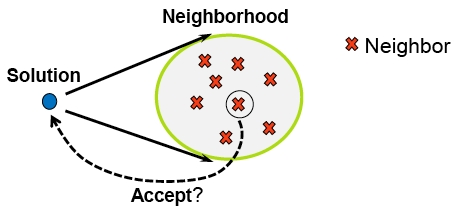
\includegraphics[width=0.7\textwidth]{images/localSearch.jpg}
			\caption{Exemple de recherche locale}
		\end{figure}
		\item \textbf{improveSolution} : le but est de  satisfaire un peu plus de clauses a chaque itérations en inversant la valeur d'une variable si elle apparait dans une clause non satisfaites de l'instance, si la nouvelle solution est meilleure que l'orignal, alors elle deviendra la solution construite par la fourmi.
	\end{itemize}
